\documentclass[10pt]{article}
\usepackage[bulgarian]{babel}
\usepackage[letterpaper,top=2cm,bottom=2cm,left=3cm,right=3cm,marginparwidth=1.75cm]{geometry}
\usepackage[style=mla,backend=biber]{biblatex}
\usepackage[colorlinks=true, allcolors=blue]{hyperref}
\usepackage{listings}
\usepackage{wrapfig}
\usepackage{graphicx}

\graphicspath{{assets/}}

\title{Курсов проект \\ {\Large Обектно-ориентирано програмиране}}
\author{Кристиян Стоименов \\ {ф.н 3MI0400121, ФМИ}}
\date{летен семестър, 2023}

\addbibresource{bibliography.bib}

\begin{document}
\maketitle

\section{Увод}

\subsection{Цел}

Целта на настоящата курсова работа е бъде реализирана програма, която да обработва и модифицира данни, подредени според разпространения текстов формат \textit{JSON} \autocite{ecma404}. Сред основните функционалности, които трябва да притежава реализираната програма е прочитане на вход и създаване на структура в паметта, следваща формата на подадените данни (т.нар \textit{parsing}), ако те са коректни. В противен случай, ако наложения формат не е спазен, то трябва грешката да бъде докладвана по начин, който предполага лесно да бъде забелязан проблемът в подадения вход. Другата основна част от функционалностите е възможността за подаване на различни команди върху вече прочетен JSON файл. Сред поддържаните команди са операции като вмъкване, премахване, извличане на стойности. Списък с всички необходими команди, както и очакваното от тях поведение, може да се намери в \textit{заданието на проекта} \autocite{json-problem}.

\section{Преглед на предметната област}

\par
JSON форматът е широко разпространен и намира приложение като начин за съхраняване на \textit{прости} данни. В него данните са наредени предимно като чифтове \textit{ключ-стойност}. В днешно време почти всеки програмен инструмент има някаква връзка с този формат данни било то възможност за негово прочитане, използване като интерпрограмен формат или създаване на изход чрез него. В случая с езика C++ според популярното хранилище за библиотеки "Conan Centre" \autocite{conan_centre} библиотеката \verb|nlohmann_json| \autocite{nlohmann_json} притежава над 400 000 отделни употреби (включва единствено случаите, когато е използвана чрез \verb|conan| \autocite{conan}).

\par
При реализацията на курсовия проект е използвана често срещаната архитектура при обработката и прочитане на текст, който следва фиксираната \textit{форма}. Тази форма обичайно се нарича граматика. Съществуват редица библиотеки, които се използват за съставяне на т.нар \textit{синтактично дърво} от подадена граматика, като тя се описва на отделен език, свързан конкретно с тази задача. Такива са например т.нар \textit{parser generators} yacc \autocite{yacc} и малко по-новия от него bison \autocite{bison}. Те от своя страна разчитат на друга сходна библиотека, която да опише отделните лексеми, които могат да се срещат сред текстовите структури на файловия формат. Такива са т.нар \textit{lexer generators} например flex \autocite{flex} и re2c \autocite{re2c}.

\section{Проектиране}

\subsection{Архитектура на проекта}

Функционалностите на проекта са разделени в два основни компонента: библиотеката \textit{json-parser} и приложението \textit{json-editor}. Библиотеката се грижи за прочитане на входни данни и създаване на структура в паметта, която да бъде семантична репрезентация на прочетеното, стига то да бъде валиден JSON. Ако подаденото на входа не е от валиден формат, библиотеката се грижи за откриването на грешката и рапортуването ѝ. Приложението използва интерфейса на библиотеката, така че да реализира поредов редактор.

\subsection{Архитектура на библиотеката}

\subsubsection{Tokenizer} \label{tokenizer-design}

\textbf{Какво е "tokenizer"?} За жалост авторът на настоящия документ не е запознат в утвърден превод на термина "tokenizer", поради което това е именно думата, която се среща в описанието на концепцията за \textit{обект}, реализиращ синтактичен анализ върху входни данни от някакъв формат (в случая JSON). Този обект борави с обекти от тип \textit{лексема}, които представляват отделени езикови единици. Това са тези части от свързан текст, които са основополагащи са по-абстрактни и по-сложни обединения в контекста на текстообработката. Често срещани лексеми са например литерали - текстови (стрингове) или числени, пунктуатори и ключови думи. JSON форматът включва няколко прости лексеми, като настоящата разбработка ги третира в четири техни вариации - \textit{число}, \textit{стринг}, \textit{пунктуатор} и \textit{ключова дума}. Основните стъпки, за които се грижи един \textit{tokenizer} включват последователно прочитане на входа и оформяне на прочетеното спрямо очаквания \textit{синтаксис} за лексемите. Фиг. \ref{fig:tokenizer_output} илюстрира изход на типа \verb|tokenizer|, имплементиран в библиотеката \textit{json-parser}, при подаване на вход \verb|{ "apple" : 3.14 }|.

\begin{figure}[h]
\centering

\includegraphics[width=.65\linewidth]{tokenizer_output.png}
\caption{Изход след изпълнение на \textit{tokenizer}}
\label{fig:tokenizer_output}
\end{figure}

Конкретната имплементация е разгледана по-подробно в подглава \ref{json-parser-impl}, посветена на \verb|json-parser| библиотеката. 

\subsubsection{Parser}
\textbf{Какво е "parser"?} За жалост, подобно на случая с \ref{tokenizer-design}, и тук няма да по-добра българска дума, с която до се опише терминът \textit{parsing}. В традиционните текстообработващи системи parser е подсистемата, която се грижи за оформяне на по-абстрактни синтактични струкури, вземайки като вход потокът от лексеми, които предоставя \textit{tokenizer}. Обикновено това се случва чрез използване на \textit{граматика}, която описва какъв е синтаксисът на валиден формат данни. В конкретиката на JSON, отделните граматични елементи са \textit{стринг}, \textit{число}, \textit{масив}, \textit{обект}, \textit{булева стойност} и \textit{празна стойност}. Граматиката на JSON е сравнително просто, което позволява просто имплементация на parser. Най-сложни от нея се явяват структурите масив и обект, които включват в себе си повече от една лексема. Фиг. \ref{fig:array_grammar} показва граматиката на масив. 

\begin{figure}[h]
\centering
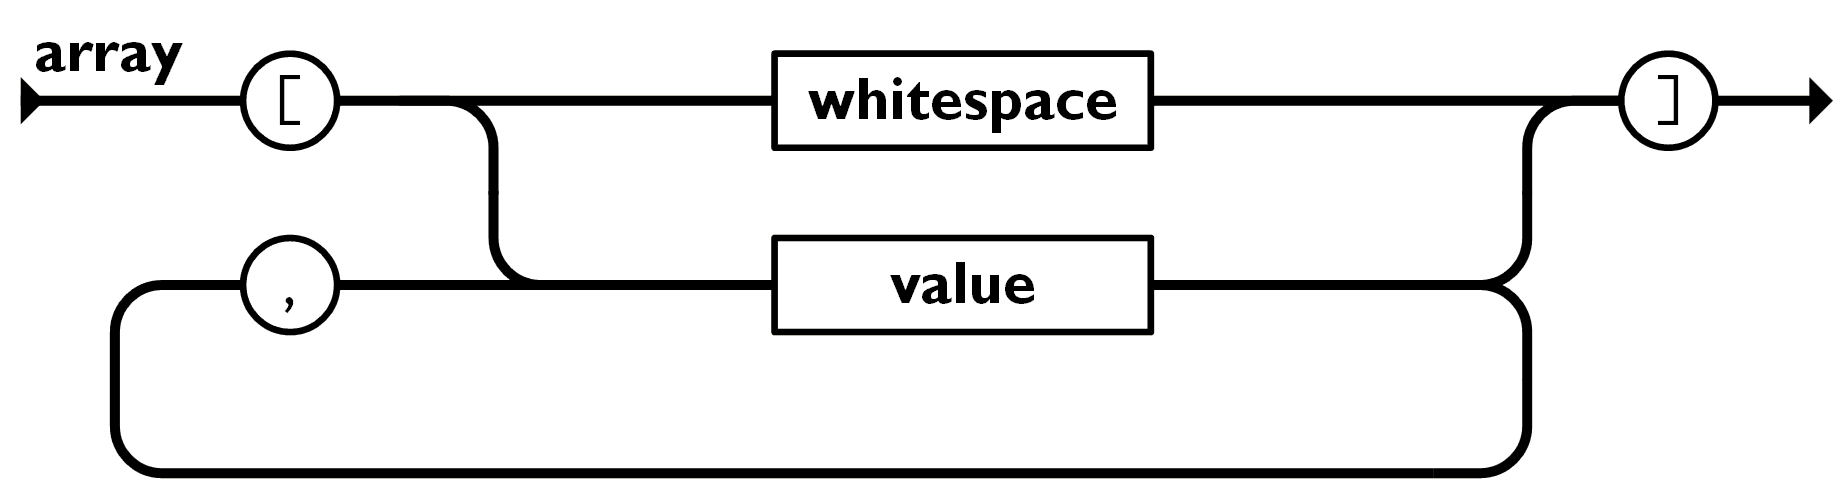
\includegraphics[width=.65\linewidth]{array_grammar.png}
\caption{Диаграма на граматиката на JSON масив \autocite{jsonorg}}
\label{fig:array_grammar}
\end{figure}

\subsubsection{Синтактично дърво}
След като бъде изпълнене процесът по \textit{parsing}, който от своя страна извиква многократно предоставения нему \textit{tokenizer}, като изход се конструира синтактично дърво. То представлява дървовидна структура, която обхваща всички синтактични елементи, срещнати в подадените входни данни. Тъй като JSON е относително прост формат, сериализиране на неговото синтактично дърво е практически същото като принтиране в JSON формат (дотолкова сходно, че JSON е популярен формат за принтиране на синтактични дървета на по-сложни езици \autocite{llvm_astdump}).

\section{Реализация}

\subsection{Библиотеката \textit{json-parser}} \label{json-parser-impl}

\par
Библиотеката \textit{json-parser} е имплементирана в директорията \verb|lib/|. Тя се компилира като статична библиотека, която в последствие трябва да бъде свързана изрично от изпълнимите файлове, които се нуждаят от нея - това включва тестовете и приложението \verb|json-editor|. Библиотеката реализира обработване (\textit{parsing}) на JSON вход от различни източници. Като своебразен изход от нея се явява типът \verb|json|, който представлява структура в паметта на съдържанието на входните данни, което позволява изпълнение на различни операции.

\par
Основните компоненти се базират на нивото на абстракция, от което разглеждаме посочените данни. Те са обхванати от типове, които биват използвани от следващите нива и \textit{стъпки от parsing процеса}. Фигура \ref{fig:parsing_steps} илюстрира стъпките, които са небходими при създаване на синтактичното дърво. Ще разгледаме типовете данни, които се използват поотделно.

\begin{wrapfigure}{r}{0.25\textwidth}
\centering
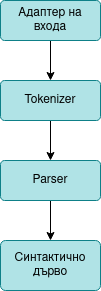
\includegraphics[width=.5\linewidth]{parsing_steps.png}
\caption{Стъпки на \textit{parsing}}
\label{fig:parsing_steps}
\end{wrapfigure}

\par
\textbf{Адаптер на входа.} Това е първата стъпка от извличането на синтактично дърво. Типовете, които се използват за това са два - \verb|ifs_input_reader| и \verb|str_input_reader| (намират се в \verb|json-parser/include/input_reader.h|). Те предоставят \textit{общ} интерфейс за прочитане на текст от респективно \verb|std::ifstream| и \verb|std::string|, което означава, че можем да използване тези типа като вход, който да съдържа валиден JSON и да може да бъде разпознат впоследствие от типа \verb|tokenizer|. Всъщност и двата адаптера наследяват общ интерфейс \verb|input_reader|, следвайки принципа на CRTP \autocite{crtp}. Основните функции, които имплементират са свързани с извличане на текст - \verb|peek()|, \verb|get()|, \verb|tell()|, \verb|seek()| и пр. Този слой е използван по-късно при реализацията на приложението \textit{json-editor}, за да се прочитат от команден ред данни, които са във валиден JSON формат.

\par
\textbf{Tokenizer.} Този тип се грижи за прочитане на входа, използвайки подаден адаптер, като извлича данни от типа \verb|token|, който представлява лексема. Той е абстрактен и се явява базов за по-конкретните лексеми, които могат да се срещнат в JSON данни. Тези лексеми са типовете \verb|token_keyword|, \verb|token_number|, \verb|token_string|, \verb|token_punct|. \verb|tokenizer| е с единствена цел да създава инстанции от итератор \verb|token_citerator|, отговарящ на изисквания на концепцията \verb|std::forward_iterator|. В него се имплементират основните функции, които да прочитат лексеми - това са функциите в семейството на \verb|consume_*()|. Те са частни са класа, като по време на \textit{parsing} се използва интерфейса на итератора.

\par
\textbf{Parser.} В това ниво на абстракция, типът \verb|parser| притежава своя инстанция на \verb|tokenizer|, която използва, за да прочита последстователно лексеми от входа, докато конструктира синтактично дърво. То е представено от типа \verb|json|, поради вече споменатото свойство на JSON формата. Основната част от работата на \verb|parser| типа се извършва от функциите в семейството на \verb|parse_*()|.

\par
\textbf{Синтактично дърво.} На този етап данните ни се представят от типа \verb|json|, като те вече са преминали целия процес на \textit{parsing} и са във вече потвърдено валидно състояние. Това позволява извършване на различни операции върху тях, като двете най-комплексни сред тях са проследяване на път в дървото и извличане на стойности, отговарящи на определено изискване. Те се имплементират респективно от \verb|follow()|, който използва типа \verb|path|, и \verb|extract_mapped_if()|, който получава предикат, на чиято база да се извърши филтрирането на съхраняваните данни.

\subsection{Приложението \textit{json-editor}}

\par
Приложението \textit{json-editor} е имплементирано в директорията \verb|app|. То се компилира като отделен изпълним файл \verb|json-editor| и се намира в \verb|${output}/app/json-editor/$|, където \verb|${output}| е зададената изходна директория. То реализира поредов редактор за файлове с JSON формат, като се базира на функционалностите предоставени от библиотеката \verb|json-parser|.

\par
Основните компоненти на приложението са класът \verb|editor| и няколко свободни функции, които имплементират съответната функционалност на поддържаните команди. В \verb|editor| се съдържа таблица от техните имена, като всяка една от тях е свързана с указател, сочещ към свободна функция, която изпълнява операцията, съответстваща на името. 
Класът има членове-функции, които добавят или премахват елементи от този вид. След като са добавени всички команди, се извиква \verb|loop|, която се грижи да последователно прочитане на вход и изпълнение на посочената команда със съответните аргументи. Входът на всяка команда е различен, което означава, че свободните функции сами се грижат са снабдяване с небходимите аргументи.

\par
Следното парче код отговаря за създаване на такъв \textit{рекатор}, който да отговаря на командите \verb|"help"|, \verb|"open"| и \verb|"close"| (\textit{из app/src/main.cpp}).

\begin{lstlisting}[language=C++]
editor cmdline { "Greetings!" };
cmdline.add_cmd("help", commands::help_cmd);
cmdline.add_cmd("open", commands::open_cmd);
cmdline.add_cmd("close", commands::close_cmd);
// [...]
cmdline.loop();
\end{lstlisting}

\par
Файлът \verb|app/src/main.cpp| създава инстанция на класа \verb|editor|, която може да изпълнява небходимите команди, посочени в заданието, а \verb|app/src/editor.h| и \verb|app/src/editor.cpp| имплементират типа \verb|editor| и свободните функции, които да изпълняват съотвените команди.

\subsection{Библиотеката \textit{mystd}}

\par
Библиотеката \verb|mystd| е имплементирана в директориите под \verb|mystd/| и има тестове в \verb|tests/mystd/|.
Основната ѝ цел е да предостави някои типове и функции от стандартната библиотека \autocite{stl}, които са използвани в реализацията на курсовия проект, но според заданието това не е разрешено. Това са типовете \verb|unique_ptr|, \verb|unordered_map| и \verb|optional|, както и някои помощни функции за работа с тях като \verb|make_unique|. Тяхната имплементация живее в именованото пространство \verb|mystd|.

\par
Важно е да се отбележи, че ефикаснотта на реализацията на тези типове не е приоритет на настояшия курсов проект. Същото важи и за придържането към стандарта на езика С++ \autocite{thestd}. Това е използвано като имплементацията на \verb|optional| се свежда до \verb|unique_ptr|, а тази на \verb|unordered_map| до две член-промеливи от тип \verb|std::vector|.

\par
В същото място, където се помещават имплементациите на типовете от \verb|mystd| се намира и файл \verb|enable.h|, който използва макро като маркер относно това дали курсовият проект да използва точно типовете от \textit{"моята стандартна библиотека"} или същинската такава. Тази функционалност на \textit{feature toggle} бе редовно използвана при реализацията на основните компоненти на проекта.

\subsection{Тестване}
По време на работата по проекта бе използвана библиотеката на съставяне на функционални тестове още наричани \textit{unit tests} \verb|gtest| \autocite{gtest}. Създадени са тестови случаи за всички компоненти на библиотеката
\verb|json-parser|, като се намират различни такива за отделните стъпи по процеса, който се изпълнява при \textit{parsing} на текстов вход. Освен тях е използван и подходът, забелязан в тестове на популярната библиотека 
\verb|nlohmann_json| \autocite{nlohmann_json}, а именно имплементираният в \verb|test_reprint|. Той предполага изпълнение на следния процес:
\begin{enumerate}
\item Прочитане на валиден JSON вход и създаване на \verb|json| обект в паметта.
\item Сериализиране на извлечения обект в отделен файл.
\item Повторно прочитане на валиден JSON вход, но този път от туко-що създадения файл, и създаване на \verb|json| обект в паметта.
\item Сериализиране на извлечения обект в отделен файл.
\item Сравняване на двата изходни файла. Очакваме те да бъдат с идентично съдържание.
\end{enumerate}

\par
В предоставения набор от тестови случаи се срещат доста такива, които очакват да се засече грешка в подадения текст. Най-много такива се виждат във файла \verb|tests/test_parser.cpp|, като там са вписани и получените грешки.

\par
Освен за библиотеката \verb|json-parser|, предоставени са тестове и за \verb|mystd|. Te също са изцяло функционални, като се базират на примерите, предоставени в документацията на техните съответни стандартни типове.

\section{Заключение}

\par
Основните цели, които са поставени пред курсовия проект, са изпълнени според посоченото задание. Въпреки това съществуват доста възможности за бъдещо подобрение на настоящата имплементация. Тук са посочени само някои от тях.

\par
Най-просто реализируемата промяна, която би донесла ползи, е изключването на макросите, които са \verb|mystd/enable.h| файла. Това би довело да използване на типовете и функциите, предоставени в стандартната библиотека, които несъмненое изпълняват задачите си по-ефикасен начин и имат несравнимо по-високо ниво на сигурност от гледна точка наличие на уязвимости и грешки.

\par
Основният фронт за подобрения е предоставеният интерфейс за типа \verb|json|. Към момента той е тромав и грозен, като за да се достъпи стойността в конкретен обект е небходимо използване на изричен \textit{cast} от вида \verb|dynamic_cast|. Несъмнено по-приятно и удобно за използване би бил конвенционалният метод с изброяване на инденксни операции, които от своя страна индексират или масив (\verb|json::array|), или обект (\verb|json::object|). Такъв например може да се види в широко разпространената библиотека \verb|nlohmann_json|. 

\par
Относно верифицарането на качество най-важното допълнение към настоящия обем тестови случаи е добавяне на т.нар \textit{fuzzy testing} \autocite{fuzzytesting}. Това е стандартен тип проверка, която се е доказала като ефективен подход за борба с проблеми свързани с текстообработка, като ежегодно се използва за намиране на проблеми в софтуер, използван от много години. За целта може да бъде използвана популярната библиотека \autocite{libFuzzer}. Това обаче
ще наложи компилиране на проекта, използвайки компилатора \verb|clang| \autocite{llvm}, докато по време на разработка бе използван \verb|gcc| \autocite{gcc}.

\printbibliography

\end{document}
